% !TEX root = main21.tex
\section{Mean volatility surface and new PCA factors}
\label{app:wide-grid-factors}
\newcommand{\WidePcaNinetyRank}{25}


\subsection{Mean and reference-date implied volatility}

Figure~\ref{fig:wide-mean-iv} shows the arithmetic mean of the wider model's
Black implied-volatility surfaces over all 891 fitted dates, with equal
weight per date. Each surface is evaluated on the same NMS $[-4,3]$ and
1--25-business-day grid, using that date's market ATM volatility scale.
This is a mean of implied volatilities, not the implied volatility of an
averaged price surface, nor an average of the DLV parameters. The right
panel is the 29 August 2025 fitted state used for the factor illustrations.
Neither panel averages simulated paths. Both include the 5\% Black
smoothing component and use business-time annualization.

\begin{figure}[H]
  \centering
  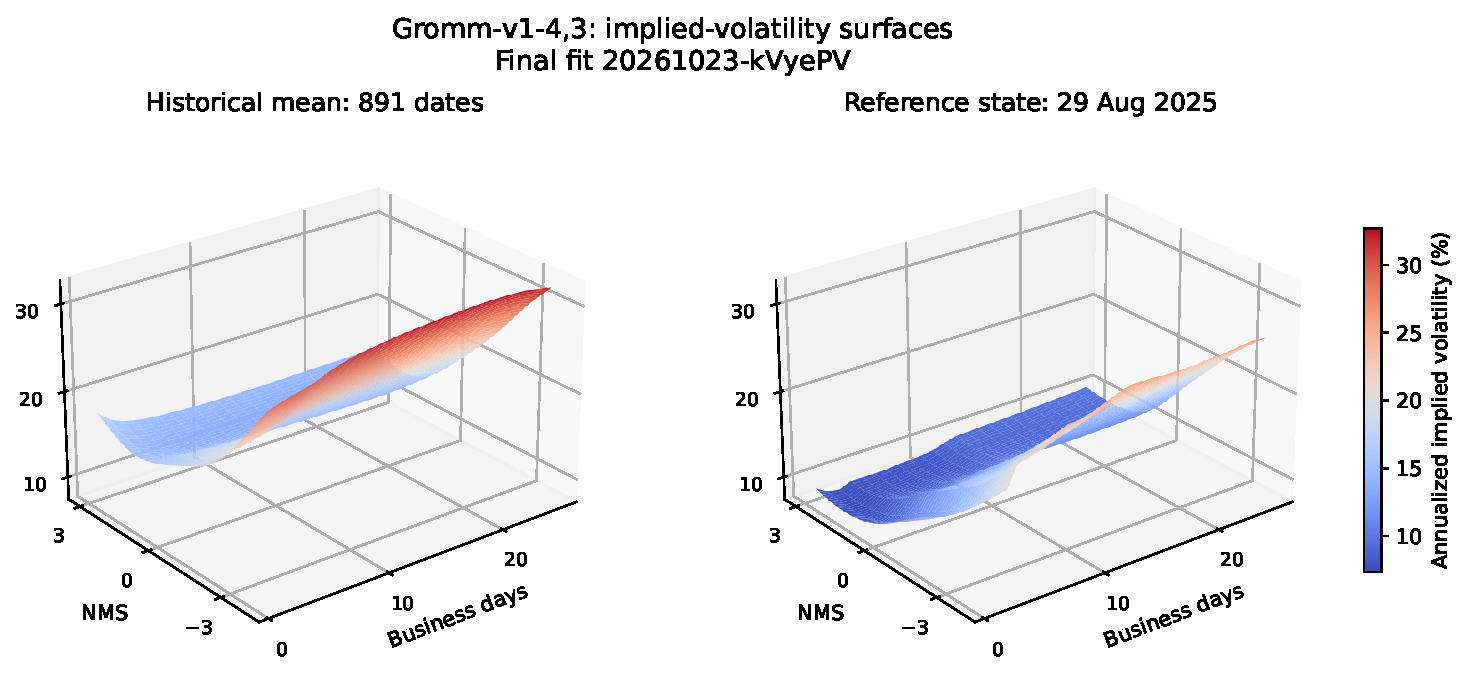
\includegraphics[width=\textwidth]{generated/wide_grid/mean_and_reference_iv.pdf}
  \caption{GROMM v1-4,3 annualized implied volatility in percent: historical
  equal-date mean (left) and reference-date state (right). Both panels use
  identical vertical and colour scales. Date-specific NMS alignment prevents
  the historical mean from mixing different standardized strikes. These are
  model surfaces over the displayed grid, including downweighted wings, not
  a claim of observed quote coverage at every plotted point.}
  \label{fig:wide-mean-iv}
\end{figure}

\subsection{Innovation spectrum}

The new factor system is the one saved by the completed wider-grid Q audit,
estimated from 710 fixed-contract historical pairs ending on 31 December
2024. The first direction is aligned to the front-spot innovation; the
remaining seven retained directions are PCs of the smoothed log-DLV
innovations after removing their spot projection. These are not PCs of
implied-volatility levels. Figure~\ref{fig:wide-pca-spectrum} reports the
spot-loading power followed by the residual covariance eigenvalues, each
divided by total smoothed innovation variance. The eight retained factors
explain \WideExplainedVariance\%; the first 90\% crossing is rank
\WidePcaNinetyRank. Eigenvalues beyond rank eight are shown for context;
those additional directions were not used in the reported Q audit.

\begin{figure}[H]
  \centering
  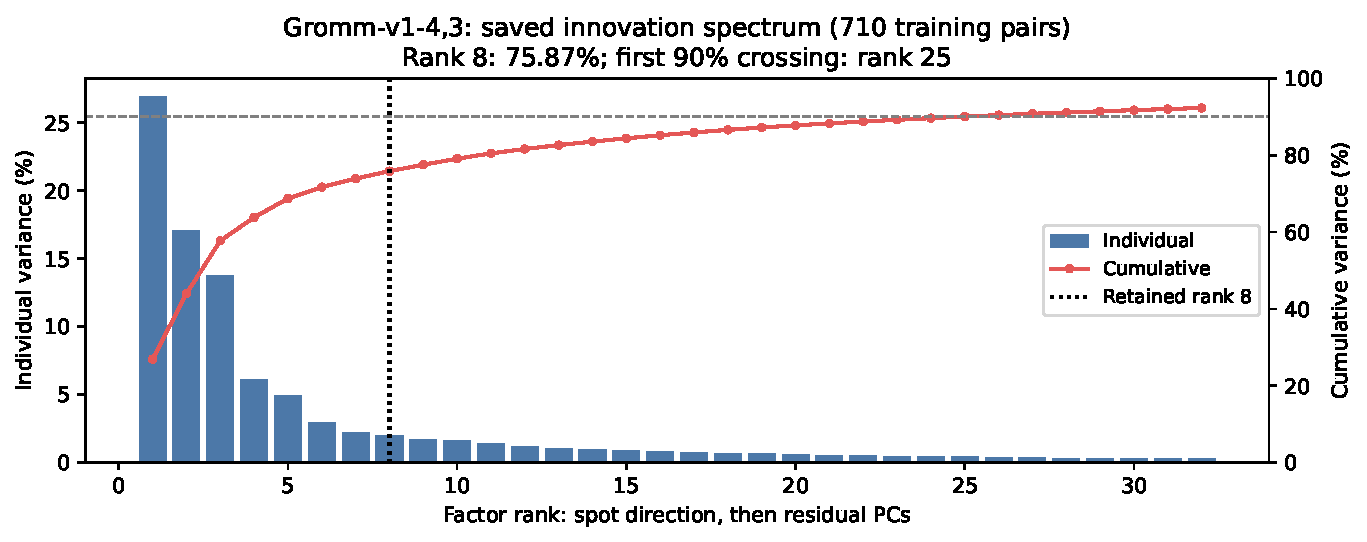
\includegraphics[width=0.94\textwidth]{generated/wide_grid/pca_explained_variance.pdf}
  \caption{New spot-oriented factor spectrum, using the saved wider-grid
  diffusion estimate. Blue bars show individual variance contributions;
  the red line is cumulative. The vertical dotted line marks the eight
  retained factors, not the rank needed to reach the horizontal 90\% line.}
  \label{fig:wide-pca-spectrum}
\end{figure}

\subsection{Implied-volatility responses of the retained factors}

At the reference-date state, each saved annualized loading $\xi_f$ is
mapped to an implied-volatility response by the same central daily shock
convention as the main paper:
\begin{equation}
  \Delta_f\sigma_{\rm imp}
  =\tfrac12\left[
    \sigma_{\rm imp}(\log\Sigma+\xi_f/\sqrt{252})
    -\sigma_{\rm imp}(\log\Sigma-\xi_f/\sqrt{252})\right].
\end{equation}
Only the future log-DLV-squared rows (days 2--25) are displaced. Spot,
the first-expiry state, and the reference-date NMS-to-strike map are held
fixed. Thus even for the spot-aligned factor this is its surface-loading
component, not a full joint spot/front-density simulation. There is no
drift or elapsed-time step in these illustrations; an equivalent measure
change leaves the illustrated diffusion directions unchanged.

\begin{figure}[H]
  \centering
  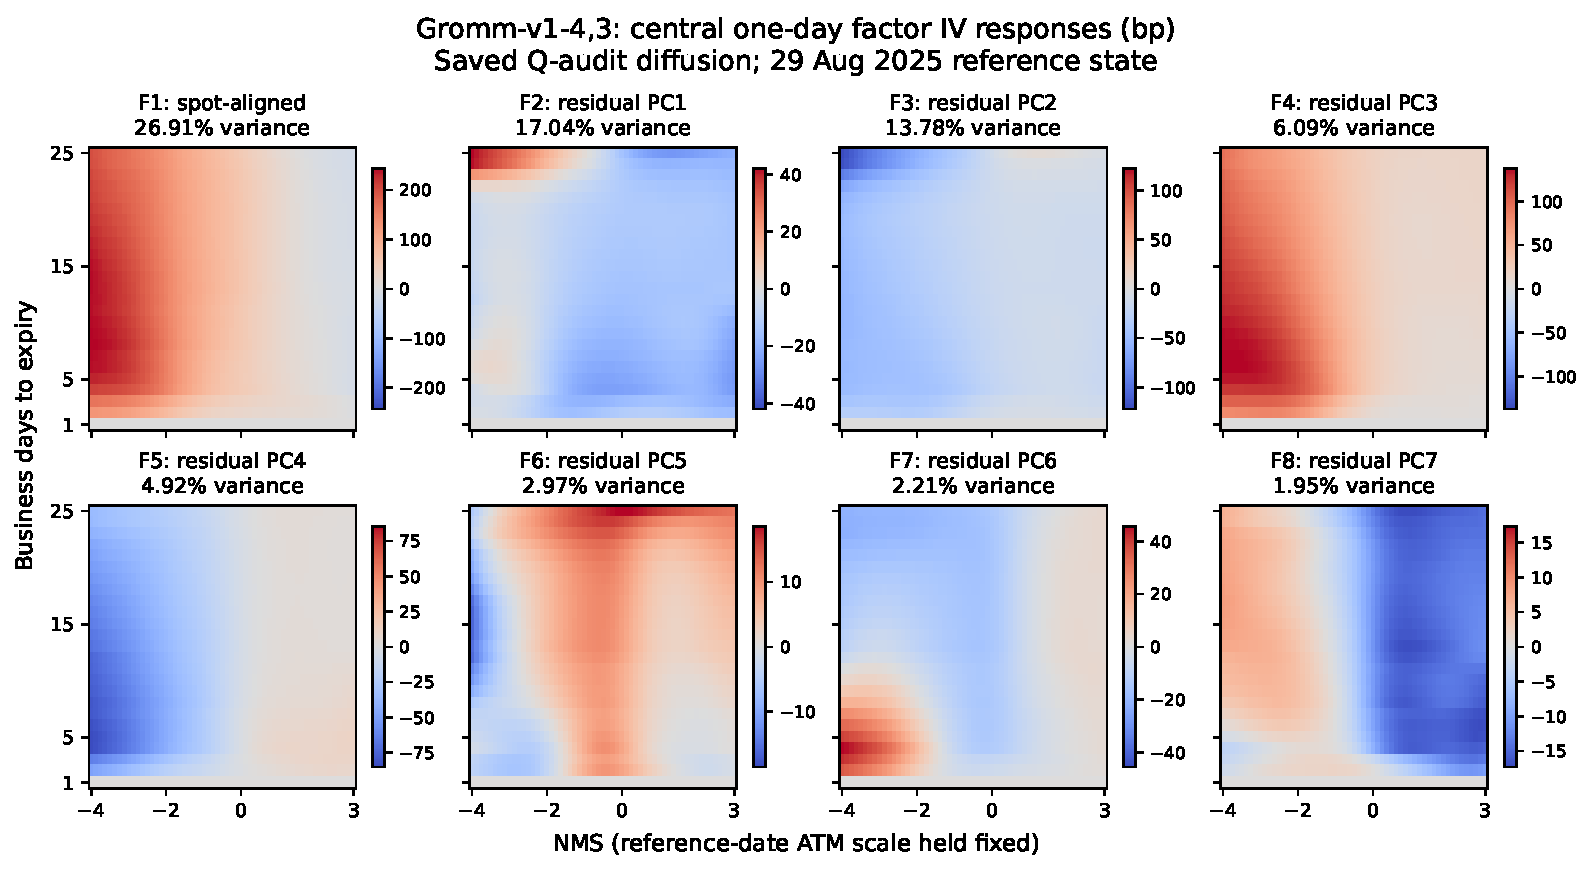
\includegraphics[width=\textwidth]{generated/wide_grid/pca_iv_responses.pdf}
  \caption{All eight new retained factors in IV coordinates. Each panel
  shows the central one-day-standard-deviation response in basis points of
  annualized IV ($1$ bp $=10^{-4}$), using its own symmetric colour scale.
  Panel percentages are contributions to total smoothed log-DLV innovation
  variance, not IV variance. F1 is spot-aligned; F2--F8 are residual PCs
  1--7. The one-day row is zero because its state is held fixed.}
  \label{fig:wide-pca-responses}
\end{figure}

The figures are regenerated by \path{quantdata/sdlv/daily/paper_wide_factors.py}.
Their plotted arrays and provenance are retained in
\path{generated/wide_grid/factor_surfaces.npz} and
\path{generated/wide_grid/factor_metrics.json}. Checkpoint identities,
reference-state reconstruction and retained variance are verified against
the same completed Q audit used in Table~\ref{tab:wide-q-audit}; no new
calibration or path simulation is performed to make these illustrations.
